%----------------------------------------------------------------------------------------
%	PACKAGES AND OTHER DOCUMENT CONFIGURATIONS
%----------------------------------------------------------------------------------------

\documentclass[fleqn,10pt]{SelfArx} % Document font size and equations flushed left

\usepackage[english]{babel} % Specify a different language here - english by default

\usepackage{lipsum} % Required to insert dummy text. To be removed otherwise

\usepackage{tikz}
\usepackage{verbatim}


%----------------------------------------------------------------------------------------
%	COLUMNS
%----------------------------------------------------------------------------------------

\setlength{\columnsep}{0.55cm} % Distance between the two columns of text
\setlength{\fboxrule}{0.75pt} % Width of the border around the abstract

%----------------------------------------------------------------------------------------
%	COLORS
%----------------------------------------------------------------------------------------

\definecolor{color1}{RGB}{0,0,90} % Color of the article title and sections
\definecolor{color2}{RGB}{0,20,20} % Color of the boxes behind the abstract and headings

%----------------------------------------------------------------------------------------
%	HYPERLINKS
%----------------------------------------------------------------------------------------

\usepackage{hyperref} % Required for hyperlinks
\hypersetup{hidelinks,colorlinks,breaklinks=true,urlcolor=color2,citecolor=color1,linkcolor=color1,bookmarksopen=false,pdftitle={Title},pdfauthor={Author}}

%----------------------------------------------------------------------------------------
%	ARTICLE INFORMATION
%----------------------------------------------------------------------------------------

%\JournalInfo{Journal, Vol. XXI, No. 1, 1-5, 2013} % Journal information
%\Archive{Additional note} % Additional notes (e.g. copyright, DOI, review/research article)

\PaperTitle{Image classification using Network in Network(NiN) architecture} % Article title

\Authors{Aditya Kant Sharma (SID: 470375615), James Macdonald (SID: 307135187)} % Authors
\affiliation{\textit{The University of Sydney, Australia}} % Author affiliation

\Keywords{Network in Network(NiN) --- Inception architecture --- Convolution Network --- Pooling Layers --- Deep Learning --- ReLU Activation --- SGD --- Dropout --- Softmax --- Batch Normalization --- Weight Normalization --- l2 Regularisation} % Keywords - if you don't want any simply remove all the text between the curly brackets
\newcommand{\keywordname}{Keywords} % Defines the keywords heading name

%----------------------------------------------------------------------------------------
%	ABSTRACT
%----------------------------------------------------------------------------------------

\Abstract{Convolution neural network (CNN, or ConvNet) are a special kind of neural networks specially designed for recognizing patterns from pixels of images. In this case study we implement convolution neural network using \textbf{Network in Network(NiN)}  architecture. The architectire used is inspired by the \textbf{inception module of GoogLeNet } where we use collaborative pooling of parallel convolution networks .
}

%----------------------------------------------------------------------------------------

\begin{document}

\flushbottom % Makes all text pages the same height

\maketitle % Print the title and abstract box

\tableofcontents % Print the contents section

\thispagestyle{empty} % Removes page numbering from the first page

%----------------------------------------------------------------------------------------
%	ARTICLE CONTENTS
%----------------------------------------------------------------------------------------

\section{Introduction} % The \section*{} command stops section numbering

%\addcontentsline{toc}{section}{Introduction} % Adds this section to the table of contents
Image classification is an important application of ConvNets. There are various architectures to design a ConvNet. The purpose of this case study is to experiment and establish an understanding of various techniques. Convolution layers and pooling layers are basic building blocks of a ConvNet. And its is crucial to understand the reason behind choosing the shape and sequence of these layers.
\newline
We have used NiN architecture where we have built parallel ConvNets and used a concatenation layer to collaborate the learning of different layers. These small NiNs are further stacked vertically with layers of NiNs. With this study we wish to demonstrate that parallel networks learn different featurs of the images and collaborating these networks outperform the traditional approach of vertically stacking convolution and pooling layers.
\newline
ConvNets can face issues with training. Training on the whole data simultaneously creates a large computational overhead for little performance gain. Training on a single observation can produce unpredictable results that do not generalise. Additionally, neural networks are prone to exploding coefficients and can suffer from the zero-gradient trap with the chosen ReLU activation. In order to address these challenges, the following features will be deployed within the neural network:
\begin{itemize}
\itemsep0em
  \item Dropout
  \item Batch normalization
  \item Weight Normalization
  \item Adam optimiser
  \item l2 Regularisation
\end{itemize}
Since this is a multiclass problem with 62 unique classes, a Softmax activation has been chosen for the output layer, allowing for the calculation and comparison of class probabilities.
%------------------------------------------------

\subsection{Data}
There are 62 classes in this dataset. The dataset has been split into training set and validation set, where the training set has 37,882 images of alphabets and numbers; while the validation set has 6,262 images. The images are of size 128*128 pixels with 3 channels.

\section{Techniques}

\subsection{Convolution Layer}
Convolution neural networks are special networks which take advantage of the fact the input consists of images. In contrast to regular neural networks ConvNets have neurons arranged in three dimensions(i.e. height,width and depth of the image). Here depths is also referred as the number of colour channels in the image.
\newline
Figure \ref{fig:convNet} gives shows that  convolution layers can be seen as hidden layer in neural networks while the output layer is a vector of size Number\_Of\_Classes arranged along depth dimension.
\begin{figure}[ht]\centering
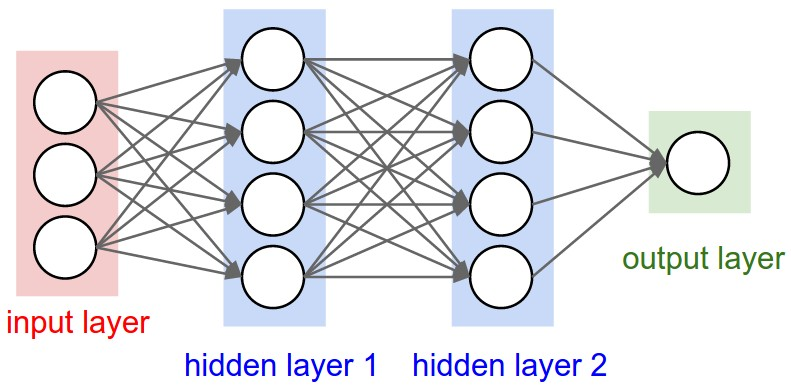
\includegraphics[width=0.49\textwidth]{neural_net}
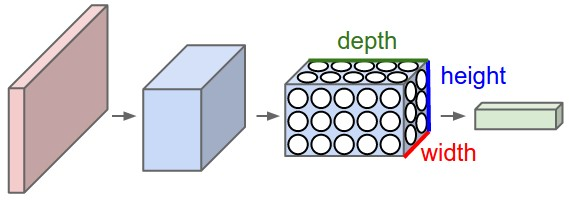
\includegraphics[width=0.49\textwidth]{cnn}
\caption{Visualisation of ConvNet}
\label{fig:convNet}
\end{figure}

\subsubsection{Building blocks of ConvNet}
As mentioned earlier we have build ConvNet using NiN architecture inspired by GoogLeNet . The three building blocks of the network are: \textbf{Convolutional Layer}, \textbf{Pooling Layer}, and \textbf{Fully-Connected Layer}(similar to regular neural networks). Details about the layers:
\begin{itemize}
\itemsep0em
  \item Convolutional Layer: Computes the output of filter applied to the local regions of the image. The filter as shown in figure \ref{fig:conv_layer} is used to extract spatial features of the image. The efficiency of feature extraction depends upon \textbf{depth}(depth of the input to the conv layer), \textbf{stride}(number of pixels by which we slide filter over the input matrix) and \textbf{zero padding}( zero padding is done along the border of the image to control the size of feature map). Since convolution is a linear operation, \textbf{ReLU activation} is often used to learn non-linearity in the data.
  \item Pooling layer: Spatial pooling(aka downsampling) reduces the dimension of each feature map while preserving the most important information. Various methods like max, average sum etc. can be used to perform spatial pooling. In ConvNets pooling layer is stacked over conv layer to reduce the length*width of the output while preserving the features learnt by different filters. Pooling layer makes the input representation smaller and manageable. Another most important feature of pooling layer is that it makes the network invariant of the the small distortions and variations in the input image.
  \item Fully connected layer: FC layers are used to compute the scores of classes. As the name suggests it is similar to normal neural networks have all neurons connected to output of previous layers. The output of FC layers is a vector of shape [1x1xNumber\_Of\_Classes].
\end{itemize}

\begin{figure}[ht]\centering
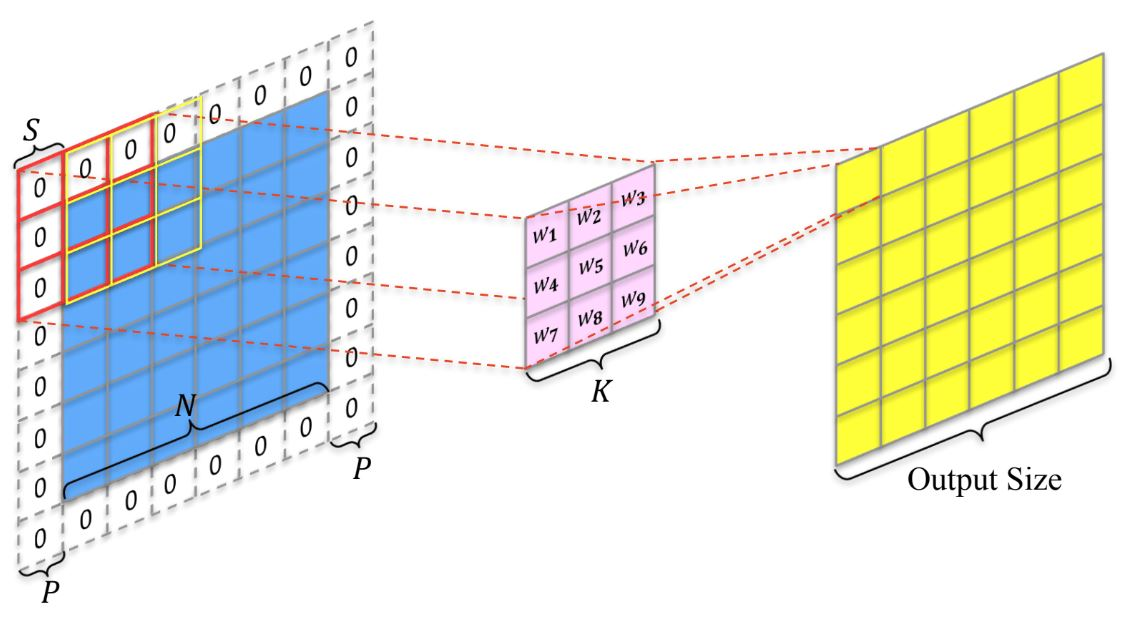
\includegraphics[width=0.49\textwidth]{conv_layer}
\caption{Convolutional Layer}
\label{fig:conv_layer}
\end{figure}

\subsection{Network Architecture}
We have used \textbf{Inception architecture} to build the ConvNet in this experiment. Filter size plays a very important role in the performance in ConvNet. But how do we decide if we should use a filter of size 3x3 or 5x5 etc. Rather we create \textbf{parallel convolutions} and concatenate the feature maps before feeding it to the next layer. The use of competitive activation units in ConvNet utilises the fact that each smaller ConvNet is capable of doing simpler tasks. Using multiple layers divide the input feature space into a number of regions which is exponentially proportional to the number of layers. Since sub-networks are trained with the samples which fall into one of the regions and as a result it becomes specialised in one set of features. Using parallel layers avoid overfitting as we concatenate the filter outputs and utilise collaborative learning of all sub networks.
\newline
If the next layer is again an inception module, the feature maps are passed through a mix of convolutions. This way the network is able to learn different features with the help of filters of different sizes and pick the best one. Having smaller convolutions help in learning local features while larger convolutions help in learning high abstracted features.
\newline
Figure \ref{fig:first_layer} shows the inception module used for the first layer. We have used a variety of convolutions: 1x1, 3x3, 5x5 convolutions along with a 3x3 max pooling layer. Since larger convolutions use more computations, we have ised \textbf{1x1 convolutions for dimensionality reduction} of the feature maps. After dimension reduction the feature map is passed to larger convolutions thus keeping the computations lower.

\begin{figure}[ht]\centering
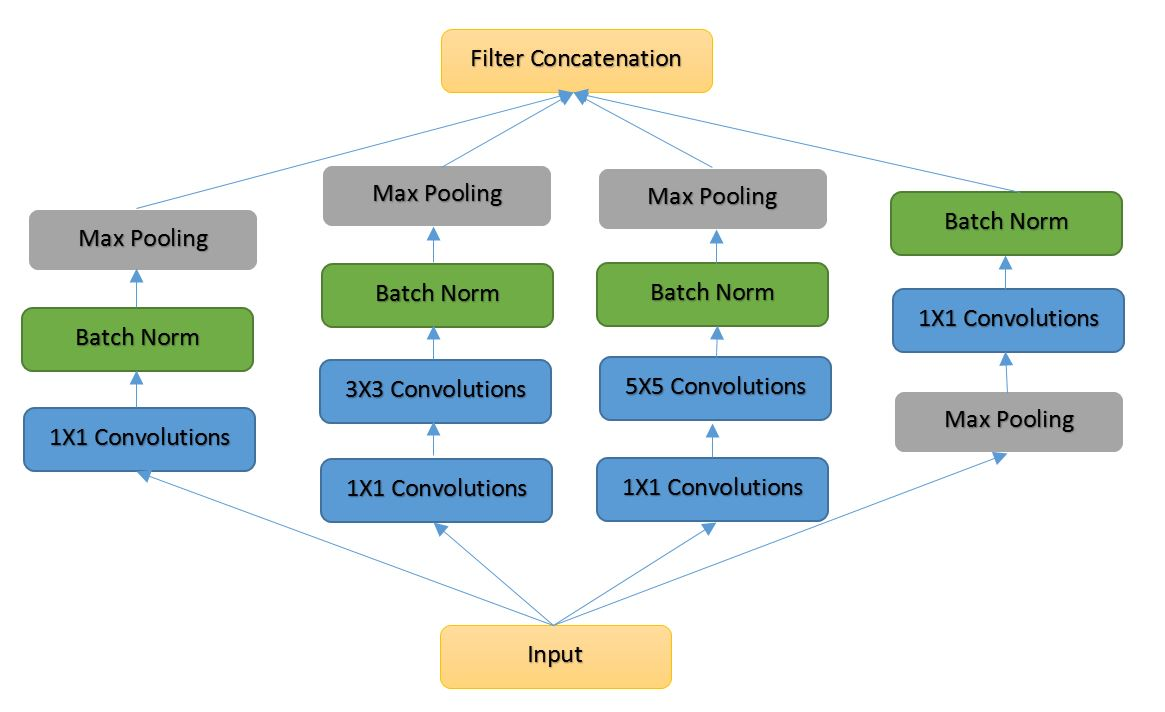
\includegraphics[width=0.49\textwidth]{first_layer}
\caption{First Inception Layer}
\label{fig:first_layer}
\end{figure}

The output of the convolutions is passed to a batch normalisation layer which improves stability and performance of the network. Similar to the concept of
normalizing the input to the network this method normalizes the input to every layer so that they have a mean output of zero and standard deviation of one. By normalizing the input before applying the activations it reduces the amount by which the hidden units output shifts. It adds few more steps to the calculation of feed-forward and back-propagation , which slows down the network. But due to normalization of inputs the network converges faster which improves overall speed of the network.each scale and also pre-conditions the model.
\newline
Finally multi scale filter outputs, weighted bu batch normalization layer are combined in the \textbf{concatenation layer} before passing on to the next layer.
\begin{figure}[ht]\centering
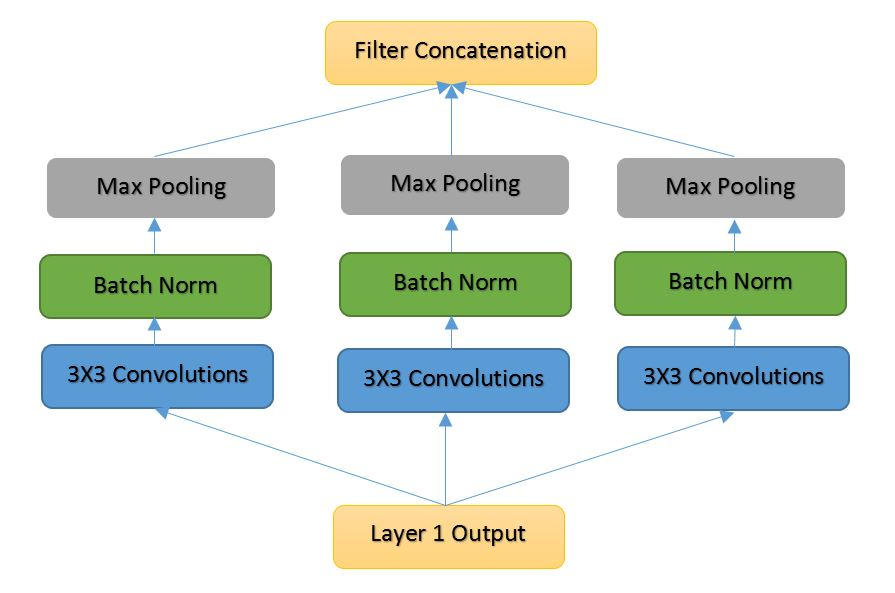
\includegraphics[width=0.49\textwidth]{second_layer}
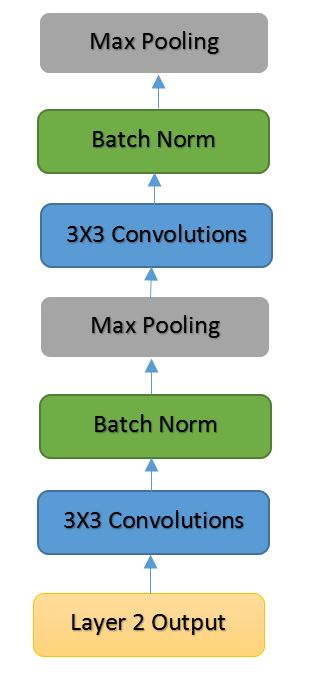
\includegraphics[width=0.20\textwidth]{3rd_4th_layer}
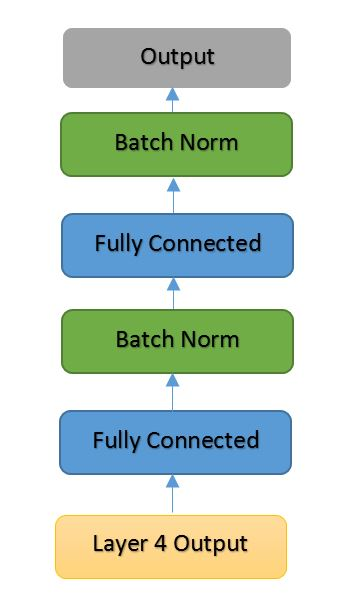
\includegraphics[width=0.20\textwidth]{final_layer}
\caption{Second Inception Layer, convolution layers and fully connected layers}
\label{fig:second_layer}
\end{figure}
We have used two inception layers to learn the low level features of the image. As shown in figure \ref{fig:second_layer} further it was stacked with two convolutional layers to recognise higher level features in the image. As the input is passed via multiple conv-layers the networks learns more complex features and increases the prediction accuracy. 
\newline
Using conv-layers the networks is able to learn both low level features and high level abstractions in the image. We use fully connected layers at the end of the network and outputs the N dimensional vector where N is the number of classes to be predicted. We have used \textbf{softmax} to find the class which is best suited to the input image. Fully connected layers connect to the out of the previous layer(which is activation map of the high level features) and finds the features which are most suitable for a particular class. FC layer uses the most correlated features for a particular class and learns weights so that we get correct probability for the different classes when it performs product of weights and output of previous layer.

\section{Experiments and results}
An experiment was run to determine the optimal settings for a number of hyperparameters. These hypereparameters are network architecture, regularization, iteration and batch size.
\newline
For the first hyperparameter, sophisticated architectures outperformed basic architectures. The introduction of multiple convolutional layers, as well as layer 'inception', raised out-of-sample performance considerably. The use of parallelized convolutions of different sizes meant that different streams could concentrate on extracting different features, and this capability was reflected in better performance.
\newline
The second hyperparameter, quickly became necessary as the network architecture exploded the count of trainable variables. In order to prevent these from overfitting, three regularization devices were used. Firstly, the model weights were penalized using L2 regularization. This suppressed extreme coefficient values in both the convolutional and fully-connected layers. L2 was eventually chosen as L1 produced sparsity, which reduced weights to zero. Secondly, batch normalization was employed in all convolutional and fully-connected layers. Batch-normalization was applied before activation functions, and was useful in preventing exploding or vanashing gradients. Lastly, a slight dropout probability was applied to the first fully-connected layer. All of these techniques improved out-of-sample performance when training accuracy approached the ceiling.
\newline
The third and fourth hyperparameters were set by trial and error. Iteration count was kept at 10,000 and batch size was 128. Lower values did not guarantee convergence and higher values resulted in overly-long training processes. Additionally, since the count of classes was so high, it was important to ensure that there was sufficient chance of all classes appearing in any given training batch.
\newline
Once the hyperparameters were established, the final version of the network was trained. The results achieved are explored below.

\subsection{Primary Metrics}
Out of sample accuracy was 86.65\%. This was a strong result but considerably lower than in-sample performance, which was 95\%. Precision was 87.55\%, Recall was 86.65\% and F1 score was 96.65\%. All results were calculated on the test set and multiclass averaging was performed according to model weights. In multi-class problems it is always harder to interpret these metrics, since there is no clear null case. This is especially true given that all classes are of the same frequency, since weighting in this instance equates to a flat average. In reality results may differ, as some letters are more common than others.

\subsection{Extensive analysis}

\subsubsection{Confusion Matrix}
The confusion matrix is an effective visualization of model performance. From the visualization provided in figure \ref{fig:confusion_matrix}, some interesting observations emerge. Firstly, while the model is very accurate there are some classes where it is quite weak. For example, for the first class recall was 69\% and precision was 79\%, both far below average. The reason for this is that the first class is the number "0", and is very similar to the letters "O" and "o". Particularly with the diversity of fonts in the dataset, the model is having difficulty discriminating between similar-looking characters. This difficulty extends to cases - there is a striking correlation in the confusion matrix as classes are misclassified with a class exactly 26 steps away. The reason for this is confusion between upper case and lower case characters - this trend stops abruptly when classes cross over into numbers. Letters like "X":"x", and "Z":"z" in particular suffered from this problem.

Both these errors show the importance of context - a human reader would not make the mistake between capital "O" and zero largely due to whether it's in a context of numbers or letters. Unfortunately context is not something available to this model, so there is a performance ceiling.\begin{figure}[ht]\centering
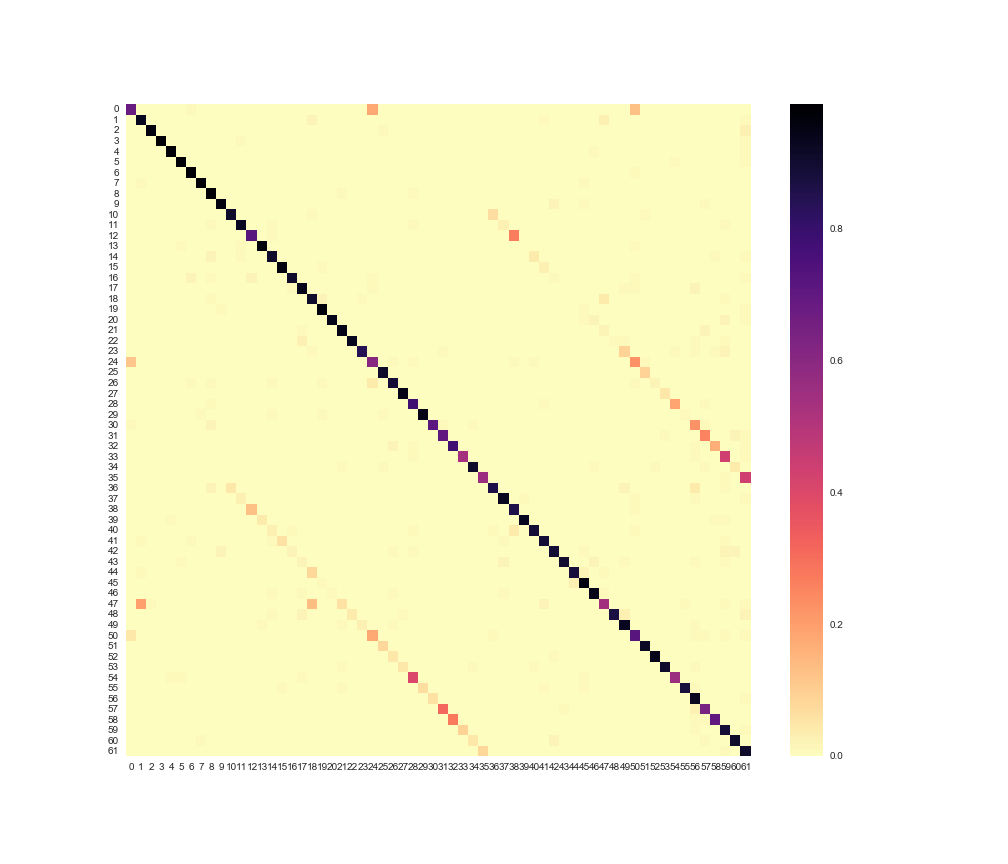
\includegraphics[width=0.49\textwidth]{confusion_matrix}
\caption{Confusion Matrix}
\label{fig:confusion_matrix}
\end{figure}
The confusion matrix (figure \ref{fig:confusion_matrix}) of the network's performance on the validation data suggests that the model struggles to recognise classes 6 and 4 - there are more incorrect predictions of data in these classes than correct ones. Most other classes, however, are predicted well and this reflects the high accuracy scores explored in the previous section.

\subsubsection{ROC and ROC-AUC}
The Response Operator Characteristics curve can be generalised to multiclass problems via a similar weighting method to the primary metrics discussed above. Weighting the AUC of individual ROCs gives an aggregated ROC AUC value of 98.15\% This is much higher than the primary metrics given above, and reflects the relative uncertainty of some of the model's predictions, where second and third place have been given a high probability too. This stems from the ambiguity in the label between similar cases and figures discussed above. The individual ROC curves are provided in figure \ref{fig:roc}.
\begin{figure}[ht]\centering
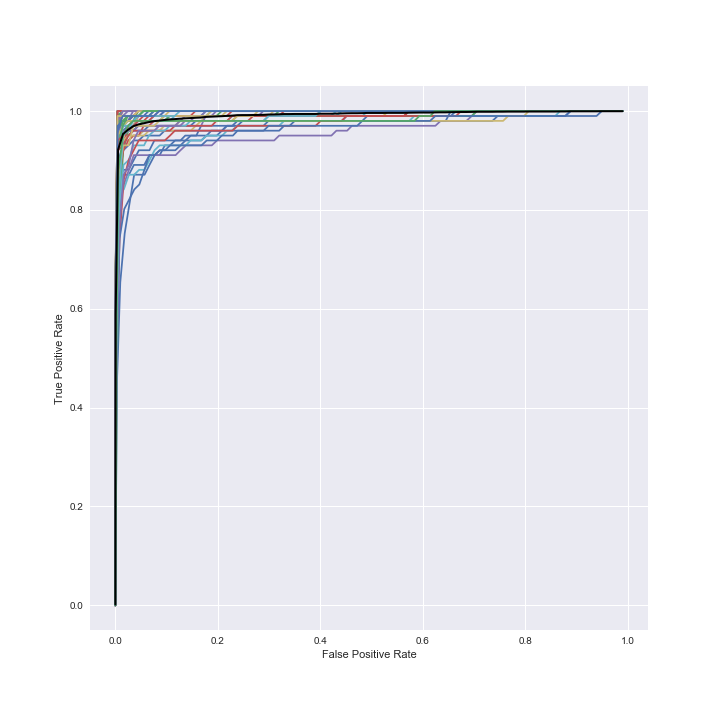
\includegraphics[width=0.49\textwidth]{roc_curves}
\caption{ROC-AUC}
\label{fig:roc}
\end{figure}


\section{Discussion}
In terms of deign of the network we can see that the use of collaborative multi-scale convolution produces more accurate results as compared to conventional ConvNets. A better performance of Inception Style model can be attributed to the collaboration of multiple parallel networks. It is important to note that the number of parameters is exponentially related to the number of features in training set. Inception style model has fewer parameters and it trains much faster using the collaborative approach.
\newline
In this dataset we have 62 classes and the number of images in training set is 38K. Considering the number of classes a higher number of images to train would help learn the features better. Also we can see a wide variety of fonts is used in the data. This increases the number of features for the model to learn. Apart from learning the shapes of alphabets the ConvNet has to learn the fonts as well. Thus increasing the training data would help in learning the rich input features.
\newline
As mentioned earlier there are similarities in the shape of few characters like 0, O, o, 1, l, L, i, I etc. These ambiguities also confuses the model and adversely affects the classification ability of the network. 

\section{Conclusions}
This study has demonstrated a functioning ConvNet with some inception modules. It has performed well on an example dataset and meet expectations based on ConvNet's performance on held out data. Batch normalisation also helped in significant increase of network performance.  
\newline
The performance of the ConvNet gives solid evidence that multiple networks are able to learn the sparsity in the data. The biggest advantage of using inception layer is significant decrease in the collaborative learning of different filters. As further study we would like to increase the depth of the networks and use filters to learn high level features to improve image classification of network.
\newline
In most of real world cases we perform image classification with the context of the image. In case of alphabets, the context is created by the letters around it. For further improvement in classification performance we would like to incorporate methods to improve feature map with the help of context and use it resolve ambiguities.

%----------------------------------------------------------------------------------------
%	REFERENCE LIST
%----------------------------------------------------------------------------------------
\begin{thebibliography}{9}
\urlstyle{same}
\bibitem{Neural Networks} 
Why neural networks
\newline
\url{https://www.doc.ic.ac.uk/~nd/surprise_96/journal/vol1/ds12/article1.html}

\bibitem{ActivationFunction} 
Activation function
\newline
\url{https://en.wikipedia.org/wiki/Activation\_function}

\bibitem{SigmoidFunction} 
Sigmoid function
\newline
\url{https://en.wikipedia.org/wiki/Sigmoid\_function}

\bibitem{CrossEntropy} 
Cross entropy
\newline
\url{https://en.wikipedia.org/wiki/Cross\_entropy}
\url{https://deepnotes.io/softmax-crossentropy}

\bibitem{SGD} 
Stochastic gradient descent
\newline
\url{https://en.wikipedia.org/wiki/Stochastic\_gradient\_descent}
\url{goo.gl/gNzHFK}

\bibitem{Precision Recall for multiclass classification} 
Precision Recall for multiclass classification
\url{goo.gl/gvMuhM}

\bibitem{Weight Normalization} 
Weight Normalization
\url{goo.gl/bd2feB}

\bibitem{Tensorflow Tutorial} 
Tensorflow 97\% MNIST result tutorial
\url{https://www.tensorflow.org/tutorials/layers}

\bibitem{hipsternet} 
Hipsternet tutorial
\url{https://github.com/wiseodd/hipsternet/}

\bibitem{COMP5329Notes} 
Lecture slides of COMP5329

 \end{thebibliography}

%----------------------------------------------------------------------------------------

\section{Appendix}
\urlstyle{same}
\subsection{Instructions on how to run code}
Following python packages are used for creation of neural network:
\begin{itemize}
\itemsep0em
  \item cv2
  \item sklearn
  \item tensorflow
  \item matplotlib
  \item numpy
\end{itemize}
We used windows machine to run this neural network. On following configuration it too around 70 minutes to execute the code:
\begin{itemize}
\itemsep0em
  \item Operating system: Linux Mint 64-bit OS
  \item CPU: Intel(R) Core(TM) i5-6600 CPU @ 3.30GHz
  \item RAM: 16.00 GB
  \item GPU: Nvidia 1070
\end{itemize}
Unzip the zip file submitted as part of assignment and follow following steps to execute the code.
\subsubsection{Data Setup}
Copy training and test data from \url{goo.gl/bY9yLd} to and unzip in Input folder.

\subsubsection{Output}
Output file with predicted labels for test file would be copied in Output folder. Name of the output file with predicted labels: test.txt.


\end{document}

